\documentclass[12pt]{article}
\renewcommand{\baselinestretch}{1.5}
\usepackage[OT4]{fontenc}
\newtheorem{define}{Definition}
\usepackage{amsmath}
\usepackage{graphicx}
\usepackage{enumitem}
\usepackage{float}

\oddsidemargin=0.15in
\evensidemargin=0.15in
\topmargin=-.5in
\textheight=9in
\textwidth=6.25in

\setlength{\oddsidemargin}{.25in}
\setlength{\evensidemargin}{.25in}
\setlength{\textwidth}{6in}
\setlength{\topmargin}{-0.4in}
\setlength{\textheight}{8.5in}

\newcommand{\handout}[5]{
	\noindent
	\begin{center}
		\framebox{
			\vbox{
				\hbox to 5.78in { {\bf #1}
					\hfill #2 }
				\vspace{4mm}
				\hbox to 5.78in { {\Large \hfill #5  \hfill} }
				\vspace{2mm}
				\hbox to 5.78in { {\it #3 \hfill #4} }
			}
		}
	\end{center}
	\vspace*{4mm}
}

\newcommand{\header}[3]{\handout{NUS CS-3235: Computer Security}{\today}{Lecturer: Reza Shokri}{Student: #2\quad#3}{#1}}

%======================================
%======================================
%======================================

\begin{document}

% Indicate your name and your student number here (e.g., A01xxx)
\header{Assignment 2 Report}{Jonathan Cheng}{A0121749A}


%======================================
\section{Buffer Overflow}

The \emph{buf} buffer is overflowed because it is filled with bytes from two other buffers, \emph{buf1} and \emph{buf2} who each (possibly) holds the same number of maximum bytes as \emph{buf}, \emph{BUFSIZE}.
Utilizing the vulnerability to pop shell is similar to tutorial 2, we fill the stack from the return address slot onwards with these 3 things in order:
\begin{enumerate}
    \item Address to gadget
    \item Address to string "\emph{\textbackslash bin\textbackslash sh}"
    \item Address to \emph{system}
\end{enumerate}
We want the gadget to pop the stack argument (address to string "\emph{\textbackslash bin\textbackslash sh}") into \emph{\$rdi}, which will cause the subsequent call the \emph{system} to pop shell.\\

The first difficulty is given the full payload, how to write the files \emph{exploit1, exploit2}. By inspection, we can alternatingly write 1 byte from the full payload to \emph{exploit1, exploit2}, starting from \emph{exploit1}. Then when the bytes are read off from the exploit files into \emph{buf}, the effect is that the payload will be written correctly into \emph{buf}. The below is the python code to do this.\\\\
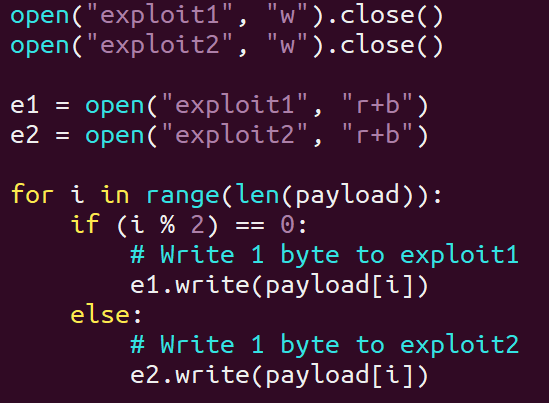
\includegraphics[scale=0.7]{./a2/buffer_overflow/alternate.PNG}\\

The next difficulty is, as mentioned in the tutorial pdf, overwriting of loop variables.\\\\
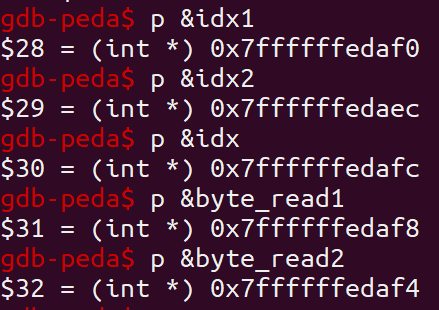
\includegraphics[scale=0.7]{./a2/buffer_overflow/extravariables.PNG}\\

The only relevant variables here are:
\begin{enumerate}
    \item \emph{byte\_read1}
    \item \emph{byte\_read2}
    \item \emph{idx}
\end{enumerate}
So to make sure that these values are consistent, our (full) payload will slot the values taken by these variables at runtime into the shellcode, like so:\\\\
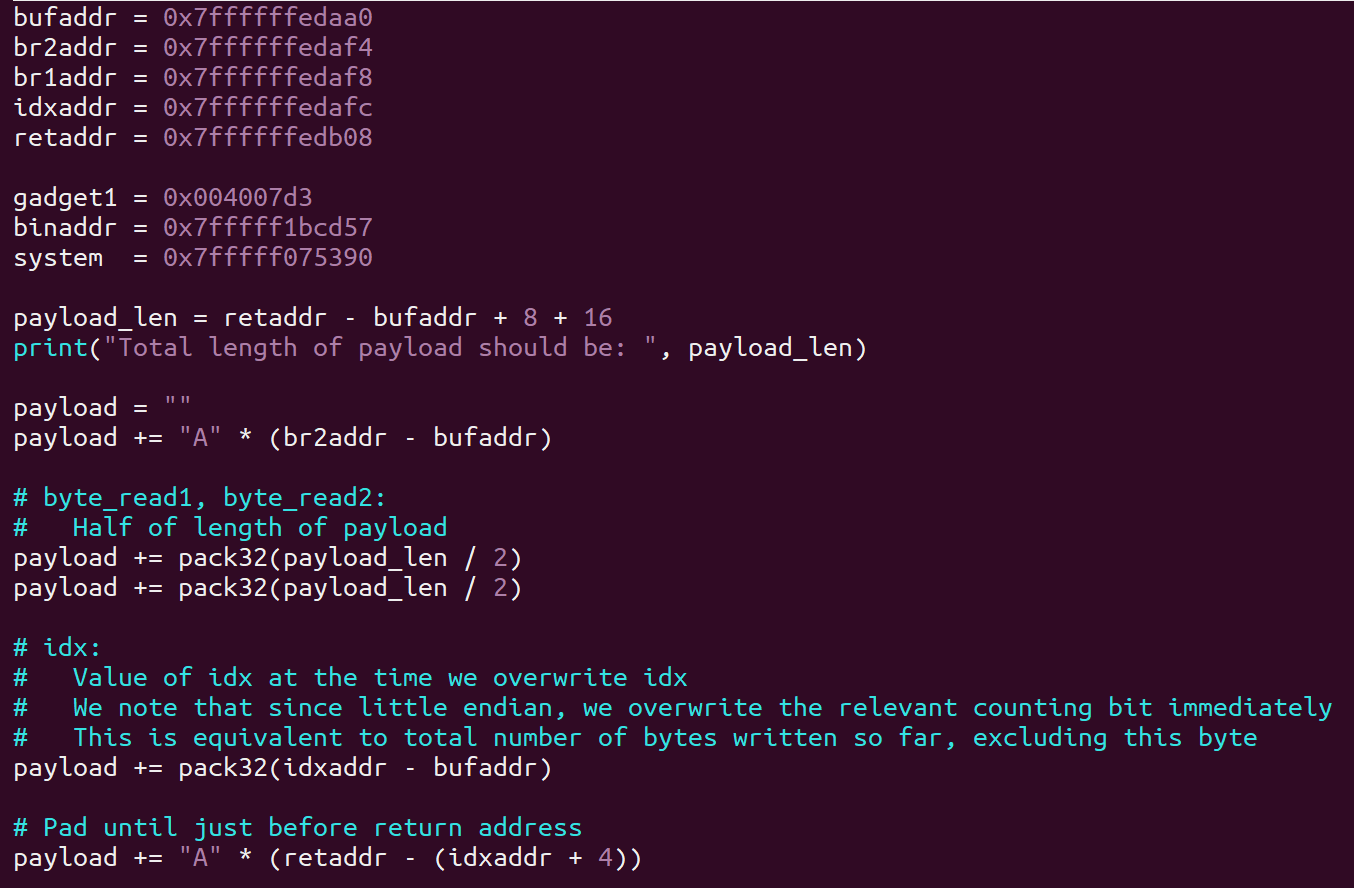
\includegraphics[scale=0.5]{./a2/buffer_overflow/extravariablesexploit.PNG}\\

The values of \emph{byte\_read1, byte\_read2} will be the half of the payload length (which corresponds to the length of files \emph{exploit1, exploit2}). The value of \emph{idx} trickier. In normal operation, it increments by 1 every time we (over)write a byte. Since we are working in a little endian system, the first byte we overwrite to \emph{idx} is the counting byte. So at that point in time, it is distance from the \emph{buf} address, excluding this first \emph{idx} byte.\\

To run the exploit, first run \emph{initexploit.py}. This will generate the files to be read. Then run the program, and shell should pop.\\

All addresses found in \emph{initexploit.py} were found using GDB, similar to tutorial 2.

%======================================

\newpage
\section{Format String Attack}





%======================================

\newpage
\section{Return-oriented Programming}



\end{document}
